\documentclass[10pt]{standalone}
\usepackage{commands}

\begin{document}
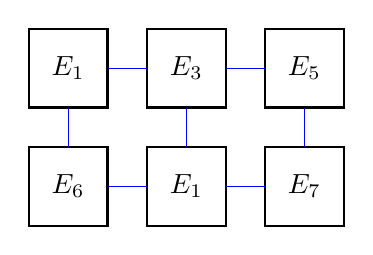
\begin{tikzpicture}
    \draw[thick] (0, 0) -- (1, 0) -- (1, 1) -- (0, 1) -- cycle;
    \draw[thick] (0+1.5, 0) -- (1+1.5, 0) -- (1+1.5, 1) -- (0+1.5, 1) -- cycle;
    \draw[thick] (0, 0+1.5) -- (1, 0+1.5) -- (1, 1+1.5) -- (0, 1+1.5) -- cycle;
    \draw[thick] (0+1.5, 0+1.5) -- (1+1.5, 0+1.5) -- (1+1.5, 1+1.5) -- (0+1.5, 1+1.5) -- cycle;
    \draw[thick] (0+3, 0+1.5) -- (1+3, 0+1.5) -- (1+3, 1+1.5) -- (0+3, 1+1.5) -- cycle;
    \draw[thick] (0+3, 0) -- (1+3, 0) -- (1+3, 1) -- (0+3, 1) -- cycle;

    \draw[blue] (0.5, 1) -- (0.5, 1.5);
    \draw[blue] (2, 1) -- (2, 1.5);
    \draw[blue] (3.5, 1) -- (3.5, 1.5);

    \draw[blue] (1, 0.5) -- (1.5, 0.5);
    \draw[blue] (2.5, 0.5) -- (3, 0.5);

    \draw[blue] (1, 2) -- (1.5, 2);
    \draw[blue] (2.5, 2) -- (3, 2);

    \node[] at (0.5, 0.5) {$E_6$};
    \node[] at (0.5, 2) {$E_1$};
    \node[] at (2, 0.5) {$E_1$};
    \node[] at (2, 2) {$E_3$};
    \node[] at (3.5, 0.5) {$E_7$};
    \node[] at (3.5, 2) {$E_5$};
\end{tikzpicture}
\end{document}